\documentclass[10pt,a4paper]{article}

\usepackage[T1]{fontenc}
\usepackage[utf8]{inputenc}
\usepackage{lmodern}
\usepackage{microtype}
\usepackage[a4paper,margin=18mm]{geometry}
\usepackage{xcolor}
\usepackage{graphicx}
\usepackage{tikz}
\usepackage{pgfplots}
\usepgfplotslibrary{groupplots}
\usepackage{caption}
\usepackage{float}
\usepackage{placeins}
\usepackage[hidelinks]{hyperref}
\usetikzlibrary{positioning,arrows.meta,shapes.geometric,fit,backgrounds,calc}
\pgfplotsset{compat=1.18}
% Shared TikZ/PGFPlots design system for the LogoLens dissertation figures.
% Load after tikz, pgfplots, xcolor and graphicx.

\definecolor{LLNavy}{HTML}{172033}
\definecolor{LLMuted}{HTML}{667085}
\definecolor{LLGrid}{HTML}{D8DEE8}
\definecolor{LLBlue}{HTML}{4C78A8}
\definecolor{LLTeal}{HTML}{16859A}
\definecolor{LLOrange}{HTML}{E28E3B}
\definecolor{LLGreen}{HTML}{5B8E55}
\definecolor{LLRed}{HTML}{C44E52}
\definecolor{LLPurple}{HTML}{7A5195}
\definecolor{LLGold}{HTML}{C99A32}

% Fixed sponsor palette used by Figures 8--10.
\definecolor{LLAon}{HTML}{0072B2}
\definecolor{LLAsc}{HTML}{E69F00}
\definecolor{LLAtm}{HTML}{009E73}
\definecolor{LLBarter}{HTML}{CC79A7}
\definecolor{LLCch}{HTML}{8C564B}
\definecolor{LLChadlaw}{HTML}{D55E00}
\definecolor{LLEllgren}{HTML}{56B4E9}
\definecolor{LLEm}{HTML}{7A5195}
\definecolor{LLFairway}{HTML}{2F4B7C}
\definecolor{LLKlg}{HTML}{F05A67}
\definecolor{LLMcp}{HTML}{00A087}
\definecolor{LLMnaClad}{HTML}{F39C34}
\definecolor{LLMnaSupport}{HTML}{6C5CE7}
\definecolor{LLPaints}{HTML}{C44E52}
\definecolor{LLRomantica}{HTML}{4E79A7}
\definecolor{LLTopNotch}{HTML}{59A14F}
\definecolor{LLFloorTonic}{HTML}{D81B60}

\tikzset{
  llbox/.style={
    rectangle,
    rounded corners=2pt,
    draw=LLNavy!65,
    line width=0.65pt,
    fill=white,
    align=center,
    inner sep=4pt,
    font=\scriptsize,
    minimum height=10mm,
    text width=23mm
  },
  lldata/.style={llbox,fill=black!3,draw=LLNavy!55},
  llblue/.style={llbox,fill=LLBlue!7,draw=LLBlue},
  llteal/.style={llbox,fill=LLTeal!7,draw=LLTeal},
  llorange/.style={llbox,fill=LLOrange!8,draw=LLOrange},
  llgreen/.style={llbox,fill=LLGreen!8,draw=LLGreen},
  llred/.style={llbox,fill=LLRed!7,draw=LLRed},
  llpurple/.style={llbox,fill=LLPurple!7,draw=LLPurple},
  llarrow/.style={-{Stealth[length=2.0mm,width=1.3mm]},line width=0.75pt,draw=LLNavy!80},
  llthinarr/.style={-{Stealth[length=1.6mm,width=1.1mm]},line width=0.55pt,draw=LLNavy!70},
  lldashed/.style={draw=LLNavy!65,dashed,rounded corners=2pt,line width=0.55pt},
  llbadge/.style={circle,fill=LLNavy,text=white,font=\scriptsize\bfseries,inner sep=1.6pt},
  llsection/.style={font=\scriptsize\bfseries,text=LLNavy,align=center},
  llnote/.style={font=\tiny,text=LLMuted,align=center},
}

\pgfplotsset{
  compat=1.18,
  llaxis/.style={
    axis line style={draw=LLNavy!55,line width=0.5pt},
    tick style={draw=LLNavy!45},
    tick label style={font=\scriptsize,text=LLNavy},
    label style={font=\scriptsize,text=LLNavy},
    title style={font=\small\bfseries,text=LLNavy},
    grid=major,
    grid style={draw=LLGrid,line width=0.35pt},
    legend style={font=\tiny,draw=LLGrid,fill=white,cells={anchor=west}},
  }
}


\captionsetup{
  font=small,
  labelfont=bf,
  labelsep=period,
  justification=justified,
  singlelinecheck=false
}

\title{LogoLens Dissertation Figures\\\large Native TikZ and PGFPlots Sources}
\author{}
\date{}

\begin{document}
\maketitle
\listoffigures
\clearpage

\begin{figure}[p]
  \centering
  \resizebox{\textwidth}{!}{% Conceptual architecture comparison: editable TikZ source.
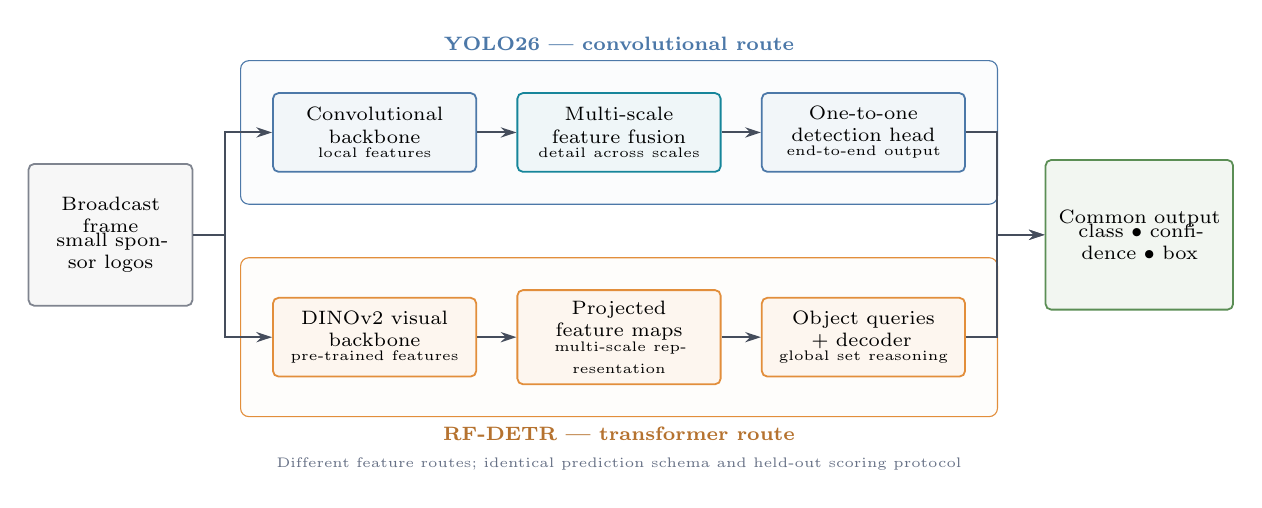
\begin{tikzpicture}[node distance=4mm and 5mm]
  \node[lldata,text width=18mm,minimum height=18mm] (input)
    {Broadcast frame\\[-1mm]\scriptsize small sponsor logos};

  \node[llblue,right=10mm of input,yshift=13mm] (yback)
    {Convolutional\\backbone\\[-1mm]\tiny local features};
  \node[llteal,right=of yback] (yfuse)
    {Multi-scale\\feature fusion\\[-1mm]\tiny detail across scales};
  \node[llblue,right=of yfuse] (yhead)
    {One-to-one\\detection head\\[-1mm]\tiny end-to-end output};

  \node[llorange,right=10mm of input,yshift=-13mm] (rback)
    {DINOv2 visual\\backbone\\[-1mm]\tiny pre-trained features};
  \node[llorange,right=of rback] (rproj)
    {Projected\\feature maps\\[-1mm]\tiny multi-scale representation};
  \node[llorange,right=of rproj] (rdec)
    {Object queries\\+ decoder\\[-1mm]\tiny global set reasoning};

  \node[llgreen,right=10mm of yhead,yshift=-13mm,text width=21mm,minimum height=19mm]
    (output) {Common output\\[-1mm]\scriptsize class $\bullet$ confidence $\bullet$ box};

  \draw[llarrow] (input.east) -- ++(4mm,0) |- (yback.west);
  \draw[llarrow] (input.east) -- ++(4mm,0) |- (rback.west);
  \draw[llarrow] (yback) -- (yfuse);
  \draw[llarrow] (yfuse) -- (yhead);
  \draw[llarrow] (rback) -- (rproj);
  \draw[llarrow] (rproj) -- (rdec);
  \draw[llarrow] (yhead.east) -- ++(4mm,0) |- (output.west);
  \draw[llarrow] (rdec.east) -- ++(4mm,0) |- (output.west);

  \begin{scope}[on background layer]
    \node[draw=LLBlue,fill=LLBlue!2,rounded corners=3pt,
      fit=(yback)(yfuse)(yhead),inner sep=4mm,
      label={[llsection,text=LLBlue]above:YOLO26 --- convolutional route}] {};
    \node[draw=LLOrange,fill=LLOrange!2,rounded corners=3pt,
      fit=(rback)(rproj)(rdec),inner sep=4mm,
      label={[llsection,text=LLOrange!80!black]below:RF-DETR --- transformer route}] {};
  \end{scope}

  \node[llnote,below=8mm of rproj]
    {Different feature routes; identical prediction schema and held-out scoring protocol};
\end{tikzpicture}
}
  \caption[YOLO26 and RF-DETR conceptual architecture]{Conceptual comparison of
  the evaluated YOLO26 and RF-DETR detection routes. Both routes return the same
  class--confidence--box schema and are evaluated using the same held-out
  protocol; the diagram is not a layer-complete network specification.}
  \label{fig:yolo-rfdetr-tikz}
\end{figure}
\clearpage

\begin{figure}[p]
  \centering
  \resizebox{0.96\textwidth}{!}{% Research framework: editable TikZ source.
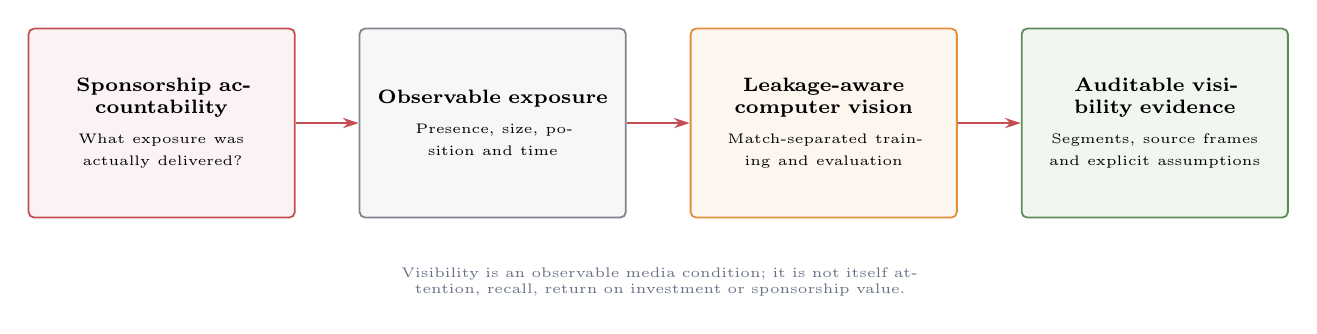
\begin{tikzpicture}[node distance=8mm]
  \node[llred,text width=31mm,minimum height=24mm] (account)
    {\textbf{Sponsorship accountability}\\[1mm]
     \tiny What exposure was actually delivered?};
  \node[lldata,right=of account,text width=31mm,minimum height=24mm] (exposure)
    {\textbf{Observable exposure}\\[1mm]
     \tiny Presence, size, position and time};
  \node[llorange,right=of exposure,text width=31mm,minimum height=24mm] (vision)
    {\textbf{Leakage-aware computer vision}\\[1mm]
     \tiny Match-separated training and evaluation};
  \node[llgreen,right=of vision,text width=31mm,minimum height=24mm] (evidence)
    {\textbf{Auditable visibility evidence}\\[1mm]
     \tiny Segments, source frames and explicit assumptions};

  \draw[llarrow,draw=LLRed] (account) -- (exposure);
  \draw[llarrow,draw=LLRed] (exposure) -- (vision);
  \draw[llarrow,draw=LLRed] (vision) -- (evidence);

  \node[llnote,below=5mm of exposure.south east,xshift=4mm,text width=82mm]
    {Visibility is an observable media condition; it is not itself attention,
     recall, return on investment or sponsorship value.};
\end{tikzpicture}
}
  \caption[Research framework]{Research framework linking sponsorship
  accountability to observable exposure, leakage-aware computer vision and
  auditable visibility evidence.}
  \label{fig:framework-tikz}
\end{figure}
\clearpage

\begin{figure}[p]
  \centering
  \resizebox{\textwidth}{!}{% Leakage-aware research design and case boundary: editable TikZ source.
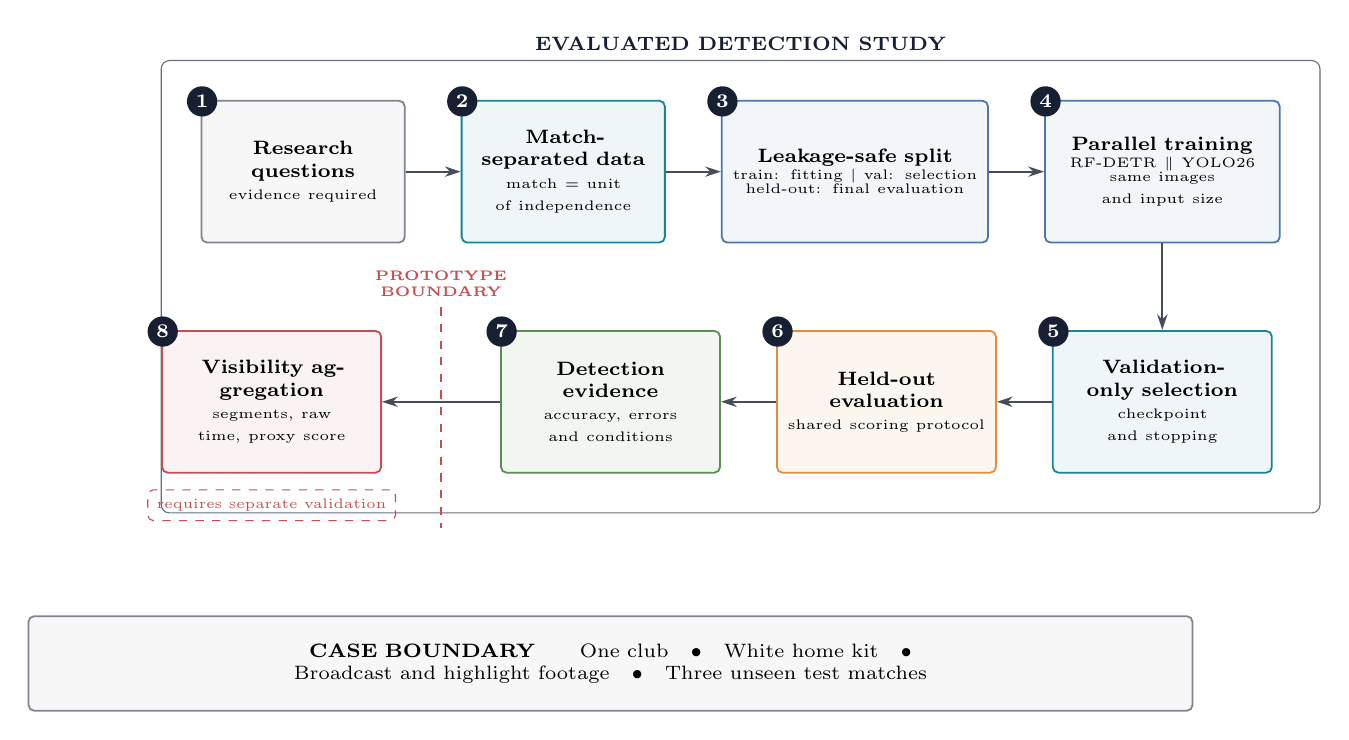
\begin{tikzpicture}[node distance=5mm and 7mm]
  \node[lldata,text width=23mm,minimum height=18mm] (rq)
    {\textbf{Research questions}\\\tiny evidence required};
  \node[llteal,right=of rq,text width=23mm,minimum height=18mm] (matches)
    {\textbf{Match-separated data}\\\tiny match = unit of independence};
  \node[llblue,right=of matches,text width=31mm,minimum height=18mm] (split)
    {\textbf{Leakage-safe split}\\\tiny train: fitting $\mid$ val: selection\\[-1mm]
     \tiny held-out: final evaluation};
  \node[llblue,right=of split,text width=27mm,minimum height=18mm] (train)
    {\textbf{Parallel training}\\\tiny RF-DETR $\parallel$ YOLO26\\[-1mm]
     \tiny same images and input size};

  \node[llteal,below=11mm of train,text width=25mm,minimum height=18mm] (select)
    {\textbf{Validation-only selection}\\\tiny checkpoint and stopping};
  \node[llorange,left=of select,text width=25mm,minimum height=18mm] (test)
    {\textbf{Held-out evaluation}\\\tiny shared scoring protocol};
  \node[llgreen,left=of test,text width=25mm,minimum height=18mm] (evidence)
    {\textbf{Detection evidence}\\\tiny accuracy, errors and conditions};
  \node[llred,left=15mm of evidence,text width=25mm,minimum height=18mm] (visibility)
    {\textbf{Visibility aggregation}\\\tiny segments, raw time, proxy score};

  \foreach \nodeName/\number in {
    rq/1,matches/2,split/3,train/4,select/5,test/6,evidence/7,visibility/8}
    \node[llbadge,above left=-1.6mm and -1.6mm of \nodeName.north west] {\number};

  \draw[llarrow] (rq) -- (matches);
  \draw[llarrow] (matches) -- (split);
  \draw[llarrow] (split) -- (train);
  \draw[llarrow] (train) -- (select);
  \draw[llarrow] (select) -- (test);
  \draw[llarrow] (test) -- (evidence);
  \draw[llarrow] (evidence) -- (visibility);

  \draw[LLRed,dashed,line width=0.7pt]
    ($(evidence.west)!0.5!(visibility.east)+(0,12mm)$) --
    ($(evidence.west)!0.5!(visibility.east)+(0,-16mm)$);
  \node[font=\tiny\bfseries,text=LLRed,align=center]
    at ($(evidence.west)!0.5!(visibility.east)+(0,15mm)$)
    {PROTOTYPE\\BOUNDARY};
  \node[draw=LLRed,dashed,rounded corners=2pt,font=\tiny,text=LLRed,
    below=2mm of visibility] {requires separate validation};

  \begin{scope}[on background layer]
    \node[draw=LLNavy!65,rounded corners=3pt,fit=(rq)(matches)(split)(train)(select)(test)(evidence),
      inner sep=5mm,label={[llsection]above:EVALUATED DETECTION STUDY}] {};
  \end{scope}

  \node[lldata,below=18mm of evidence,text width=145mm,minimum height=12mm] (boundary)
    {\textbf{CASE BOUNDARY}\qquad
     One club\quad$\bullet$\quad White home kit\quad$\bullet$\quad
     Broadcast and highlight footage\quad$\bullet$\quad Three unseen test matches};
\end{tikzpicture}
}
  \caption[Research design and case boundary]{Leakage-aware research design and
  case boundary. Training, validation and held-out matches have non-overlapping
  roles; visibility aggregation remains outside the validated detection study.}
  \label{fig:design-tikz}
\end{figure}
\clearpage

\begin{figure}[p]
  \centering
  % Dataset split and leakage diagnostic: editable PGFPlots source.
\begin{minipage}[t]{0.49\linewidth}
\centering
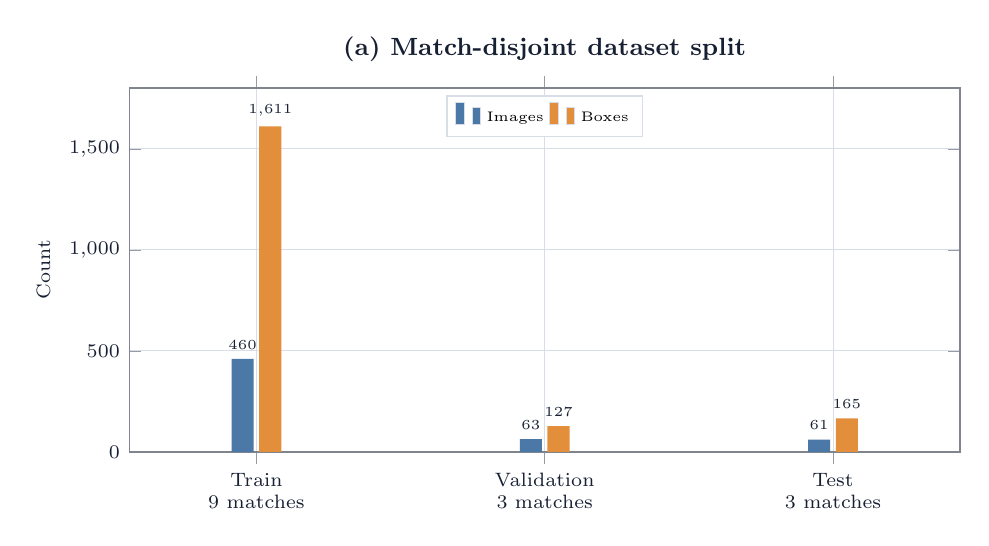
\begin{tikzpicture}
\begin{axis}[
  llaxis,
  width=\linewidth,
  height=62mm,
  ybar,
  bar width=8pt,
  ymin=0,
  ymax=1800,
  ylabel={Count},
  symbolic x coords={Train,Validation,Test},
  xtick=data,
  xticklabels={\shortstack{Train\\9 matches},\shortstack{Validation\\3 matches},\shortstack{Test\\3 matches}},
  enlarge x limits=0.22,
  nodes near coords,
  every node near coord/.append style={font=\tiny,text=LLNavy},
  legend columns=2,
  legend style={at={(0.5,0.98)},anchor=north},
  title={(a) Match-disjoint dataset split},
]
  \addplot[fill=LLBlue,draw=none] coordinates {
    (Train,460) (Validation,63) (Test,61)
  };
  \addplot[fill=LLOrange,draw=none] coordinates {
    (Train,1611) (Validation,127) (Test,165)
  };
  \legend{Images,Boxes}
\end{axis}
\end{tikzpicture}
\end{minipage}\hfill
\begin{minipage}[t]{0.49\linewidth}
\centering
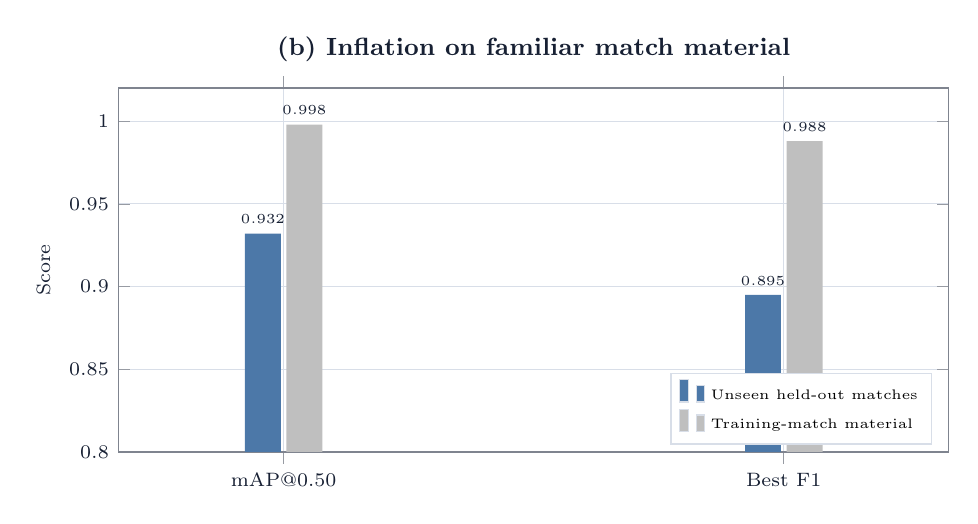
\begin{tikzpicture}
\begin{axis}[
  llaxis,
  width=\linewidth,
  height=62mm,
  ybar,
  bar width=13pt,
  ymin=0.80,
  ymax=1.02,
  ylabel={Score},
  symbolic x coords={mAP50,F1},
  xtick=data,
  xticklabels={mAP@0.50,Best F1},
  enlarge x limits=0.33,
  nodes near coords,
  every node near coord/.append style={font=\tiny,text=LLNavy,/pgf/number format/fixed,/pgf/number format/precision=3},
  legend columns=1,
  legend style={at={(0.98,0.02)},anchor=south east},
  title={(b) Inflation on familiar match material},
]
  \addplot[fill=LLBlue,draw=none] coordinates {(mAP50,0.932) (F1,0.895)};
  \addplot[fill=black!25,draw=none] coordinates {(mAP50,0.998) (F1,0.988)};
  \legend{Unseen held-out matches,Training-match material}
\end{axis}
\end{tikzpicture}
\end{minipage}

  \caption[Dataset split and temporal leakage]{Match-disjoint dataset composition
  and measured inflation on familiar match material. Familiar-material scores are
  a leakage diagnostic rather than a generalisation result.}
  \label{fig:split-leakage-pgf}
\end{figure}
\clearpage

\begin{figure}[p]
  \centering
  \resizebox{\textwidth}{!}{% LogoLens processing pipeline: editable TikZ source.
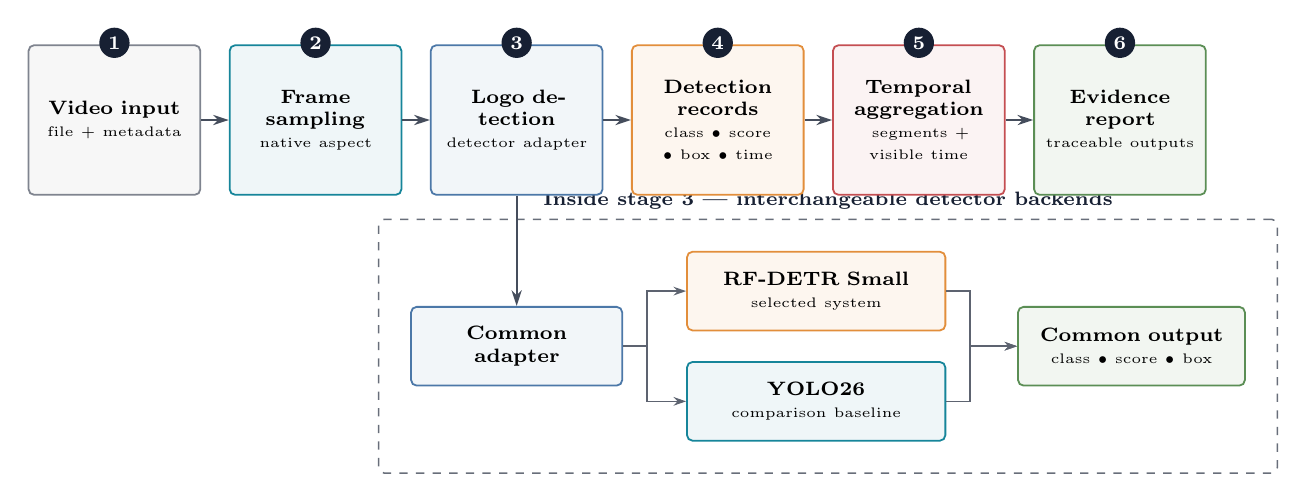
\begin{tikzpicture}[node distance=3.5mm]
  \node[lldata,text width=19mm,minimum height=19mm] (video)
    {\textbf{Video input}\\\tiny file + metadata};
  \node[llteal,right=of video,text width=19mm,minimum height=19mm] (sample)
    {\textbf{Frame sampling}\\\tiny native aspect};
  \node[llblue,right=of sample,text width=19mm,minimum height=19mm] (detect)
    {\textbf{Logo detection}\\\tiny detector adapter};
  \node[llorange,right=of detect,text width=19mm,minimum height=19mm] (records)
    {\textbf{Detection records}\\\tiny class $\bullet$ score $\bullet$ box $\bullet$ time};
  \node[llred,right=of records,text width=19mm,minimum height=19mm] (aggregate)
    {\textbf{Temporal aggregation}\\\tiny segments + visible time};
  \node[llgreen,right=of aggregate,text width=19mm,minimum height=19mm] (report)
    {\textbf{Evidence report}\\\tiny traceable outputs};

  \foreach \nodeName/\number in {video/1,sample/2,detect/3,records/4,aggregate/5,report/6}
    \node[llbadge,above=-1.8mm of \nodeName.north] {\number};

  \draw[llarrow] (video) -- (sample);
  \draw[llarrow] (sample) -- (detect);
  \draw[llarrow] (detect) -- (records);
  \draw[llarrow] (records) -- (aggregate);
  \draw[llarrow] (aggregate) -- (report);

  \node[llblue,below=14mm of detect,text width=24mm] (adapter)
    {\textbf{Common adapter}};
  \node[llorange,right=8mm of adapter,yshift=7mm,text width=30mm] (rfdetr)
    {\textbf{RF-DETR Small}\\\tiny selected system};
  \node[llteal,right=8mm of adapter,yshift=-7mm,text width=30mm] (yolo)
    {\textbf{YOLO26}\\\tiny comparison baseline};
  \node[llgreen,right=9mm of rfdetr,yshift=-7mm,text width=26mm] (common)
    {\textbf{Common output}\\\tiny class $\bullet$ score $\bullet$ box};

  \draw[llarrow] (detect.south) -- (adapter.north);
  \draw[llthinarr] (adapter.east) -- ++(3mm,0) |- (rfdetr.west);
  \draw[llthinarr] (adapter.east) -- ++(3mm,0) |- (yolo.west);
  \draw[llthinarr] (rfdetr.east) -- ++(3mm,0) |- (common.west);
  \draw[llthinarr] (yolo.east) -- ++(3mm,0) |- (common.west);

  \begin{scope}[on background layer]
    \node[lldashed,fit=(adapter)(rfdetr)(yolo)(common),inner sep=4mm,
      label={[llsection]above:Inside stage 3 --- interchangeable detector backends}] {};
  \end{scope}
\end{tikzpicture}
}
  \caption[LogoLens system architecture]{LogoLens processing pipeline. RF-DETR
  Small and YOLO26 sit behind a common adapter and return one detection-record
  schema, preserving traceability from report to source frame.}
  \label{fig:system-tikz}
\end{figure}
\clearpage

\begin{figure}[p]
  \centering
  \resizebox{\textwidth}{!}{% Visibility quality and duration measurement: editable TikZ source.
% A deliberately linear reading path avoids ambiguous branches and crossings.
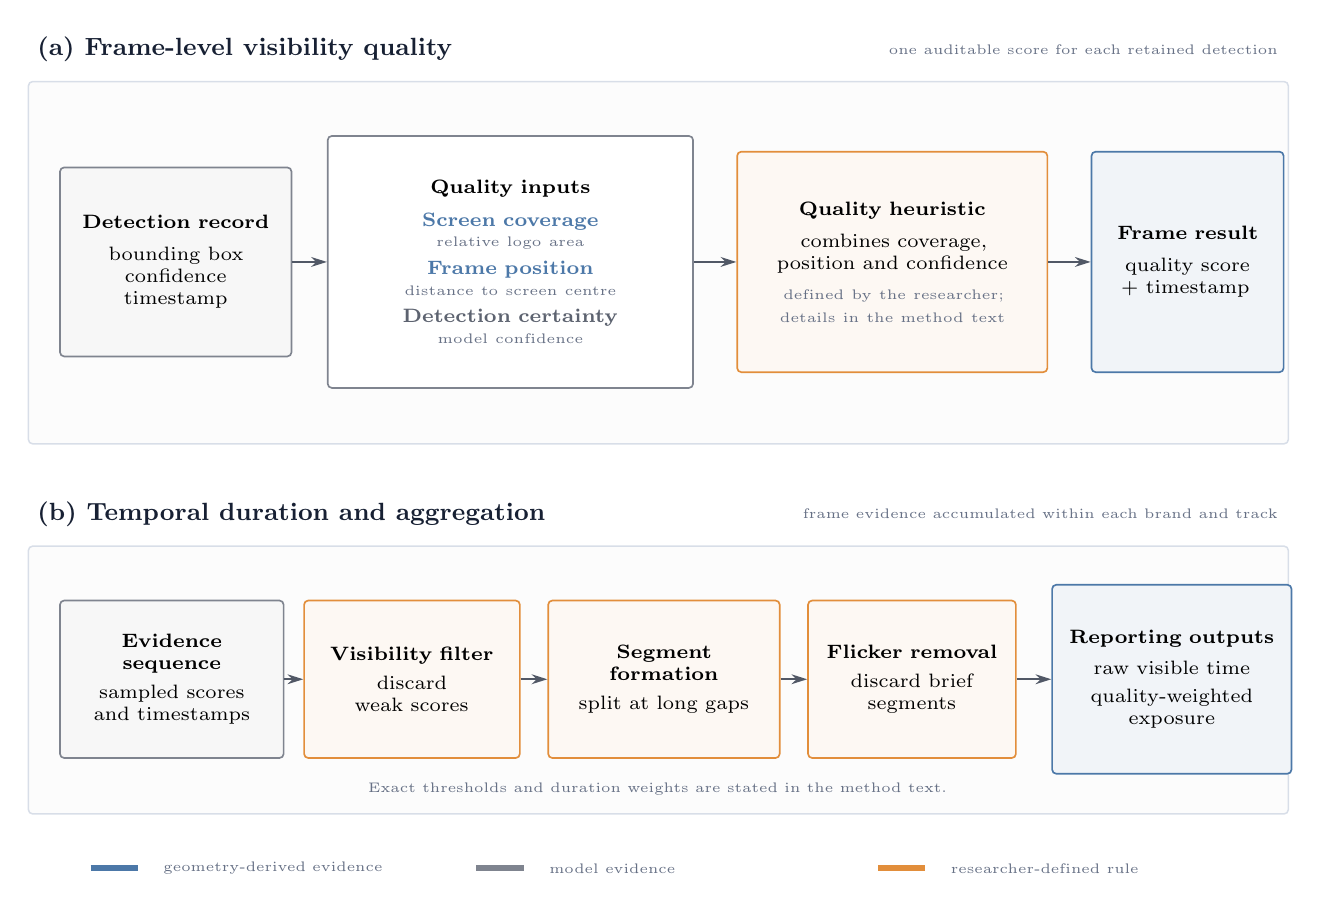
\begin{tikzpicture}[x=1mm,y=1mm]
  \tikzset{
    vispanel/.style={
      draw=LLGrid,
      line width=0.55pt,
      rounded corners=1.5pt,
      fill=black!1
    },
    visbox/.style={
      draw=LLNavy!55,
      line width=0.6pt,
      rounded corners=1.5pt,
      fill=white,
      align=center,
      inner sep=2.2mm,
      font=\scriptsize
    },
    vismodel/.style={visbox,draw=LLNavy!55,fill=black!3},
    visrule/.style={visbox,draw=LLOrange,fill=LLOrange!6},
    visoutput/.style={visbox,draw=LLBlue,fill=LLBlue!8},
    visarrow/.style={
      -{Stealth[length=2.0mm,width=1.25mm]},
      draw=LLNavy!75,
      line width=0.7pt
    },
    vistitle/.style={font=\small\bfseries,text=LLNavy,anchor=west},
    vissubtitle/.style={font=\tiny,text=LLMuted,anchor=west}
  }

  % ------------------------------------------------------------------
  % Panel A: one linear frame-level path
  % ------------------------------------------------------------------
  \node[vistitle] at (0,96) {(a) Frame-level visibility quality};
  \node[vissubtitle,anchor=east] at (160,96)
    {one auditable score for each retained detection};
  \node[vispanel,minimum width=160mm,minimum height=46mm,anchor=north west]
    at (0,92) {};

  \node[vismodel,text width=25mm,minimum height=24mm,anchor=west] (record) at (4,69)
    {\textbf{Detection record}\\[1.2mm]
     bounding box\\confidence\\timestamp};

  \node[visbox,draw=LLNavy!55,text width=42mm,minimum height=32mm,anchor=west]
    (inputs) at (38,69)
    {\textbf{Quality inputs}\\[1.3mm]
     \textcolor{LLBlue}{\textbf{Screen coverage}}\\[-0.2mm]
     \textcolor{LLMuted}{\tiny relative logo area}\\[0.7mm]
     \textcolor{LLBlue}{\textbf{Frame position}}\\[-0.2mm]
     \textcolor{LLMuted}{\tiny distance to screen centre}\\[0.7mm]
     \textcolor{LLNavy!70}{\textbf{Detection certainty}}\\[-0.2mm]
     \textcolor{LLMuted}{\tiny model confidence}};

  \node[visrule,text width=35mm,minimum height=28mm,anchor=west] (score) at (90,69)
    {\textbf{Quality heuristic}\\[1.3mm]
     combines coverage,\\position and confidence\\[1mm]
     \textcolor{LLMuted}{\tiny defined by the researcher; details in the method text}};

  \node[visoutput,text width=20mm,minimum height=28mm,anchor=west] (frameout) at (135,69)
    {\textbf{Frame result}\\[1.2mm]
     quality score\\+ timestamp};

  \draw[visarrow] (record.east) -- (inputs.west);
  \draw[visarrow] (inputs.east) -- (score.west);
  \draw[visarrow] (score.east) -- (frameout.west);

  % ------------------------------------------------------------------
  % Panel B: one linear temporal path
  % ------------------------------------------------------------------
  \node[vistitle] at (0,37) {(b) Temporal duration and aggregation};
  \node[vissubtitle,anchor=east] at (160,37)
    {frame evidence accumulated within each brand and track};
  \node[vispanel,minimum width=160mm,minimum height=34mm,anchor=north west]
    at (0,33) {};

  \node[vismodel,text width=24mm,minimum height=20mm,anchor=west] (sequence) at (4,16)
    {\textbf{Evidence sequence}\\[0.8mm]
     sampled scores\\and timestamps};
  \node[visrule,text width=23mm,minimum height=20mm,anchor=west] (floor) at (35,16)
    {\textbf{Visibility filter}\\[0.8mm]
     discard weak scores};
  \node[visrule,text width=25mm,minimum height=20mm,anchor=west] (segment) at (66,16)
    {\textbf{Segment formation}\\[0.8mm]
     split at long gaps};
  \node[visrule,text width=22mm,minimum height=20mm,anchor=west] (flicker) at (99,16)
    {\textbf{Flicker removal}\\[0.8mm]
     discard brief segments};
  \node[visoutput,text width=26mm,minimum height=24mm,anchor=west] (outputs) at (130,16)
    {\textbf{Reporting outputs}\\[1.1mm]
     raw visible time\\[0.7mm]
     quality-weighted exposure};

  \draw[visarrow] (sequence.east) -- (floor.west);
  \draw[visarrow] (floor.east) -- (segment.west);
  \draw[visarrow] (segment.east) -- (flicker.west);
  \draw[visarrow] (flicker.east) -- (outputs.west);

  \node[vissubtitle,anchor=center] at (80,2)
    {Exact thresholds and duration weights are stated in the method text.};

  % Evidence-status key.
  \draw[LLBlue,line width=2.2pt] (8,-8) -- (14,-8);
  \node[vissubtitle] at (16,-8) {geometry-derived evidence};
  \draw[LLNavy!55,line width=2.2pt] (57,-8) -- (63,-8);
  \node[vissubtitle] at (65,-8) {model evidence};
  \draw[LLOrange,line width=2.2pt] (108,-8) -- (114,-8);
  \node[vissubtitle] at (116,-8) {researcher-defined rule};
\end{tikzpicture}
}
  \caption[Visibility quality and duration aggregation]{Visibility quality and
  duration measurement. Panel (a) converts box geometry and detector confidence
  into a frame-level heuristic; panel (b) filters and groups ordered scores into
  segments before reporting raw visible time and quality-weighted exposure.}
  \label{fig:visibility-tikz}
\end{figure}
\clearpage

\begin{figure}[p]
  \centering
  % RF-DETR training trajectory and held-out evidence. All charts are native
% PGFPlots/TikZ and read directly from the retained data files.
\newcommand{\lltrainHeader}[2]{%
  {\scriptsize\bfseries #1}\hfill
  {\tiny\color{LLMuted}#2}\par\vspace{0.7mm}}

% ---------------------------------------------------------------------------
% Tier 1: both axes live in one groupplot, which guarantees identical vertical
% alignment, plot height and x-axis baseline.
\begin{tikzpicture}
\begin{groupplot}[
  group style={group size=2 by 1,horizontal sep=13mm},
  llaxis,
  width=74mm,
  height=48mm,
  xmin=0,xmax=51,
  xtick={0,10,20,30,36,40,51},
  xlabel={Epoch},
  title style={font=\scriptsize\bfseries,text=LLNavy},
]
\nextgroupplot[
  title={(a) Composite detection loss},
  ymin=0,ymax=38,
  ytick={0,5,10,20,30},
  ylabel={Composite loss},
  legend columns=2,
  legend style={at={(0.98,0.98)},anchor=north east},
  unbounded coords=jump,
]
  \addplot[LLBlue,line width=0.9pt,no marks]
    table[col sep=comma,x=epoch,y=train_loss]{data/fig07_training.csv};
  \addplot[LLOrange,line width=0.9pt,no marks]
    table[col sep=comma,x=epoch,y=val_loss]{data/fig07_training.csv};
  \draw[LLGreen,densely dotted,line width=0.9pt]
    (axis cs:36,0) -- (axis cs:36,38);
  \legend{Training,Validation}

\nextgroupplot[
  title={(b) Validation and checkpoint selection},
  ymin=0,ymax=0.80,
  ytick={0,0.2,0.4,0.6,0.8},
  ylabel={Validation mAP@[0.50:0.95]},
  legend columns=2,
  legend style={at={(0.98,0.04)},anchor=south east},
]
  \addplot[LLBlue,line width=0.9pt,no marks]
    table[col sep=comma,x=epoch,y=val_map]{data/fig07_training.csv};
  \addplot[LLOrange,line width=0.9pt,no marks]
    table[col sep=comma,x=epoch,y=ema_map]{data/fig07_training.csv};
  \draw[LLGreen,densely dotted,line width=0.9pt]
    (axis cs:36,0) -- (axis cs:36,0.80);
  \addplot[only marks,mark=*,mark size=2.0pt,LLGreen]
    coordinates {(36,0.741244)};
  \node[font=\tiny\bfseries,text=LLNavy,fill=white,draw=LLGrid,
    rounded corners=1pt,inner sep=1.5pt,anchor=south east]
    at (axis cs:34.5,0.625) {epoch 36: 0.741};
  \legend{Validation,EMA validation}
\end{groupplot}
\end{tikzpicture}

\vspace{3.2mm}

% ---------------------------------------------------------------------------
% Tier 2: full-width operating-point matrix. Numeric class IDs replace rotated
% brand names; the mapping is printed separately to eliminate label collisions.
\lltrainHeader{(c) Held-out operating-point confusion}{confidence $\geq0.35$; IoU $\geq0.50$}
\newcommand{\llcmcell}[4]{%
  \ifnum#1=15
    \fill[LLOrange!#3] (#1,#2) rectangle ++(1,1);
  \else
    \ifnum#2=0
      \fill[LLOrange!#3] (#1,#2) rectangle ++(1,1);
    \else
      \fill[LLBlue!#3] (#1,#2) rectangle ++(1,1);
    \fi
  \fi
  \node[font=\tiny,text=\ifnum#3>55 white\else LLNavy\fi]
    at (#1+0.5,#2+0.5) {#4};}
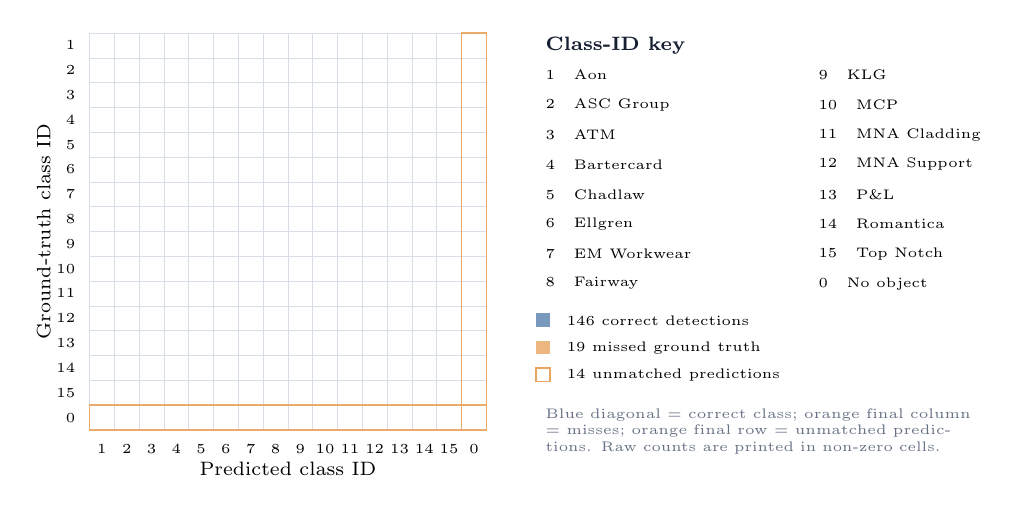
\begin{tikzpicture}[x=3.15mm,y=3.15mm]
  \fill[white] (0,0) rectangle (16,16);
  \draw[LLGrid,line width=0.22pt,step=1] (0,0) grid (16,16);
  % Auto-generated non-zero confusion-matrix cells: x, y, intensity, raw count.
\llcmcell{0}{15}{86}{17}
\llcmcell{15}{15}{19}{1}
\llcmcell{1}{14}{90}{11}
\llcmcell{2}{13}{78}{5}
\llcmcell{15}{13}{28}{1}
\llcmcell{3}{12}{60}{3}
\llcmcell{15}{12}{45}{2}
\llcmcell{15}{11}{90}{1}
\llcmcell{5}{10}{90}{7}
\llcmcell{6}{9}{78}{5}
\llcmcell{15}{9}{28}{1}
\llcmcell{7}{8}{90}{3}
\llcmcell{8}{7}{80}{27}
\llcmcell{15}{7}{25}{4}
\llcmcell{9}{6}{76}{22}
\llcmcell{15}{6}{29}{5}
\llcmcell{10}{5}{90}{2}
\llcmcell{15}{4}{90}{1}
\llcmcell{12}{3}{86}{17}
\llcmcell{15}{3}{19}{1}
\llcmcell{13}{2}{84}{12}
\llcmcell{15}{2}{21}{1}
\llcmcell{14}{1}{85}{15}
\llcmcell{15}{1}{20}{1}
\llcmcell{0}{0}{20}{1}
\llcmcell{1}{0}{36}{4}
\llcmcell{5}{0}{26}{2}
\llcmcell{6}{0}{20}{1}
\llcmcell{7}{0}{20}{1}
\llcmcell{8}{0}{20}{1}
\llcmcell{13}{0}{26}{2}
\llcmcell{14}{0}{26}{2}

  \draw[LLOrange!75,line width=0.55pt] (15,0) rectangle (16,16);
  \draw[LLOrange!75,line width=0.55pt] (0,0) rectangle (16,1);

  \foreach \pos/\id in {
    0.5/1,1.5/2,2.5/3,3.5/4,4.5/5,5.5/6,6.5/7,7.5/8,
    8.5/9,9.5/10,10.5/11,11.5/12,12.5/13,13.5/14,14.5/15,15.5/0}
    \node[font=\tiny,anchor=north] at (\pos,-0.18) {\id};

  \foreach \pos/\id in {
    15.5/1,14.5/2,13.5/3,12.5/4,11.5/5,10.5/6,9.5/7,8.5/8,
    7.5/9,6.5/10,5.5/11,4.5/12,3.5/13,2.5/14,1.5/15,0.5/0}
    \node[font=\tiny,anchor=east] at (-0.18,\pos) {\id};

  \node[font=\scriptsize] at (8,-1.55) {Predicted class ID};
  \node[font=\scriptsize,rotate=90] at (-1.85,8) {Ground-truth class ID};

  \node[font=\scriptsize\bfseries,text=LLNavy,anchor=west]
    at (18.0,15.5) {Class-ID key};
  \foreach \yy/\id/\name in {
    14.3/1/Aon,13.1/2/ASC Group,11.9/3/ATM,10.7/4/Bartercard,
    9.5/5/Chadlaw,8.3/6/Ellgren,7.1/7/EM Workwear,5.9/8/Fairway}
    \node[font=\tiny,anchor=west] at (18.0,\yy) {\id\quad \name};
  \foreach \yy/\id/\name in {
    14.3/9/KLG,13.1/10/MCP,11.9/11/MNA Cladding,10.7/12/MNA Support,
    9.5/13/P\&L,8.3/14/Romantica,7.1/15/Top Notch,5.9/0/No object}
    \node[font=\tiny,anchor=west] at (29.0,\yy) {\id\quad \name};

  \fill[LLBlue!75] (18.0,4.15) rectangle ++(0.55,0.55);
  \node[font=\tiny,anchor=west] at (18.85,4.42) {146 correct detections};
  \fill[LLOrange!65] (18.0,3.05) rectangle ++(0.55,0.55);
  \node[font=\tiny,anchor=west] at (18.85,3.32) {19 missed ground truth};
  \draw[LLOrange!80,line width=0.65pt] (18.0,1.95) rectangle ++(0.55,0.55);
  \node[font=\tiny,anchor=west] at (18.85,2.22) {14 unmatched predictions};
  \node[font=\tiny,text=LLMuted,anchor=north west,align=left,text width=55mm]
    at (18.0,1.25)
    {Blue diagonal = correct class; orange final column = misses; orange final row = unmatched predictions. Raw counts are printed in non-zero cells.};
\end{tikzpicture}

\vspace{3.2mm}

% ---------------------------------------------------------------------------
% Tier 3: full-width class-level AP chart. Labels sit outside bar ends on an
% opaque white background so neither bars nor the mean line cross the values.
\lltrainHeader{(d) Per-brand held-out AP@0.50}{all-class mean 0.933; support in parentheses; CCH omitted ($n=0$)}
\begin{tikzpicture}
\begin{axis}[
  llaxis,
  width=0.82\linewidth,
  height=64mm,
  xbar,
  xmin=0,xmax=1.08,
  ymin=-0.6,ymax=14.7,
  xlabel={AP@0.50},
  ytick={0,...,14},
  yticklabels={
    ATM (6),EM Workwear (6),Bartercard (5),MCP (27),Fairway (3),
    Romantica (13),Top Notch (16),P\&L (18),ASC Group (11),
    Ellgren (7),KLG (31),Aon (18),Chadlaw (1),MNA Support (1),MNA Cladding (2)
  },
  yticklabel style={font=\tiny},
  bar width=2.6mm,
  point meta=x,
]
  \addplot[fill=LLBlue,draw=none,bar shift=0pt,
    nodes near coords={\pgfmathprintnumber[fixed,precision=3,zerofill]{\pgfplotspointmeta}},
    every node near coord/.append style={font=\tiny,text=LLNavy,anchor=west,
      xshift=1.5pt,fill=white,inner sep=0.7pt}]
    table[col sep=comma,x=ap50,y=index]{data/fig07_per_brand_stable.csv};
  \addplot[fill=black!28,draw=none,bar shift=0pt,
    nodes near coords={\pgfmathprintnumber[fixed,precision=3,zerofill]{\pgfplotspointmeta}},
    every node near coord/.append style={font=\tiny,text=LLNavy,anchor=west,
      xshift=1.5pt,fill=white,inner sep=0.7pt}]
    table[col sep=comma,x=ap50,y=index]{data/fig07_per_brand_sparse.csv};
\end{axis}
\end{tikzpicture}

{\tiny\color{LLMuted}
\textcolor{LLBlue}{\rule{1.5mm}{1.5mm}} $n\geq5$ boxes\quad
\textcolor{black!35}{\rule{1.5mm}{1.5mm}} $n<5$ boxes}

  \caption[RF-DETR training and held-out evidence]{RF-DETR Small training and
  held-out evidence: loss trajectory, validation checkpoint selection,
  operating-point confusion matrix and per-brand AP@0.50. Grey bars indicate
  classes with fewer than five held-out boxes.}
  \label{fig:training-pgf}
\end{figure}
\clearpage

\begin{figure}[p]
  \centering
  % Qualitative occlusion examples: layout and annotations are TikZ; source frames remain raster evidence.
\newcommand{\lloccPanel}[9]{%
  {\scriptsize\bfseries #1}\hfill{\tiny\color{LLMuted}#2}\par\vspace{0.6mm}
  \begin{tikzpicture}
    \node[anchor=south west,inner sep=0] (img) at (0,0)
      {\includegraphics[width=\linewidth]{#3}};
    \begin{scope}[
      shift={(img.south west)},
      x={($(img.south east)-(img.south west)$)},
      y={($(img.north west)-(img.south west)$)}]
      \draw[#5,line width=0.9pt] (#6,#7) rectangle (#8,#9);
      \node[anchor=south east,inner sep=1.2pt,fill=white,draw=#5,line width=0.8pt]
        (zoom) at (0.985,0.025) {\includegraphics[width=0.29\linewidth]{#4}};
      % White underlay keeps the callout legible over a busy broadcast frame.
      \draw[white,line width=2.2pt] (#8,#9) -- (zoom.north west);
      \draw[white,line width=2.2pt] (#8,#7) -- (zoom.south west);
      \draw[#5,line width=0.8pt] (#8,#9) -- (zoom.north west);
      \draw[#5,line width=0.8pt] (#8,#7) -- (zoom.south west);
    \end{scope}
  \end{tikzpicture}}

\newcommand{\lloccMissPanel}[9]{%
  {\scriptsize\bfseries #1}\hfill{\tiny\color{LLMuted}#2}\par\vspace{0.6mm}
  \begin{tikzpicture}
    \node[anchor=south west,inner sep=0] (img) at (0,0)
      {\includegraphics[width=\linewidth]{#3}};
    \begin{scope}[
      shift={(img.south west)},
      x={($(img.south east)-(img.south west)$)},
      y={($(img.north west)-(img.south west)$)}]
      \draw[#5,dashed,line width=0.9pt] (#6,#7) rectangle (#8,#9);
      \node[anchor=south east,inner sep=1.2pt,fill=white,draw=#5,line width=0.8pt]
        (zoom) at (0.985,0.025) {\includegraphics[width=0.29\linewidth]{#4}};
      \draw[white,line width=2.2pt] (#8,#9) -- (zoom.north west);
      \draw[white,line width=2.2pt] (#8,#7) -- (zoom.south west);
      \draw[#5,dashed,line width=0.8pt] (#8,#9) -- (zoom.north west);
      \draw[#5,dashed,line width=0.8pt] (#8,#7) -- (zoom.south west);
    \end{scope}
  \end{tikzpicture}}

\begin{minipage}[t]{0.495\linewidth}
\lloccPanel
  {A --- Clear: Top Notch}{detected; confidence 0.915}
  {assets/fig08_A_source.jpg}{assets/fig08_A_crop.png}{LLTopNotch}
  {0.507896}{0.719639}{0.558500}{0.771676}
\end{minipage}\hfill
\begin{minipage}[t]{0.495\linewidth}
\lloccPanel
  {B --- Partially occluded: Aon}{detected; confidence 0.780}
  {assets/fig08_B_source.jpg}{assets/fig08_B_crop.png}{LLAon}
  {0.516508}{0.232382}{0.541168}{0.270792}
\end{minipage}

\vspace{2mm}

\begin{minipage}[t]{0.495\linewidth}
\lloccMissPanel
  {C --- Partially occluded: Aon}{missed; no prediction}
  {assets/fig08_C_source.jpg}{assets/fig08_C_crop.png}{LLAon}
  {0.442637}{0.325319}{0.465465}{0.365229}
\end{minipage}\hfill
\begin{minipage}[t]{0.495\linewidth}
\lloccPanel
  {D --- Heavily occluded: Fairway}{detected; confidence 0.351}
  {assets/fig08_D_source.jpg}{assets/fig08_D_crop.png}{LLFairway}
  {0.737661}{0.389333}{0.772974}{0.435685}
\end{minipage}

\vspace{1mm}
{\tiny\color{LLMuted}
Solid box = matched ground truth \quad$\mid$\quad
Dashed box = missed ground truth \quad$\mid$\quad
Colour = sponsor class.}

  \caption[Qualitative held-out occlusion examples]{Qualitative held-out cases
  across clear, partially occluded and heavily occluded conditions. The examples
  illustrate detector behaviour and do not constitute an aggregate occlusion
  benchmark.}
  \label{fig:occlusion-tikz}
\end{figure}
\clearpage

\begin{figure}[p]
  \centering
  % Representative held-out outcomes. Layout, boxes and callouts are native TikZ;
% the four source frames and two detail crops remain natural-colour raster evidence.
\tikzset{
  tp/.style={solid},
  fp/.style={densely dashed},
  miss/.style={dash pattern=on 4pt off 2pt}
}

% Box coordinates are normalised to the displayed source frame. The label
% argument is retained because the overlay files are also machine-readable,
% but success panels deliberately omit in-frame labels to avoid visual clutter.
\newcommand{\lldetbox}[7]{%
  \draw[#5,#7,line width=1.0pt] (#1,#2) rectangle (#3,#4);}

\newcommand{\lldetHeader}[2]{%
  {\scriptsize\bfseries #1}\hfill
  {\tiny\color{LLMuted}#2}\par\vspace{0.7mm}}

\newcommand{\lldetPanel}[4]{%
  \lldetHeader{#1}{#2}
  \begin{tikzpicture}
    \node[anchor=south west,inner sep=0] (img) at (0,0)
      {\includegraphics[width=\linewidth]{#3}};
    \begin{scope}[
      shift={(img.south west)},
      x={($(img.south east)-(img.south west)$)},
      y={($(img.north west)-(img.south west)$)}]
      \input{#4}
    \end{scope}
  \end{tikzpicture}}

% Row 1: successful outcomes. Only class-coloured boxes are shown; the summary
% line carries the evidential count and avoids covering the sponsor marks.
\begin{minipage}[t]{0.495\linewidth}
\lldetPanel
  {(a) Complete seven-logo detection}{7/7 ground-truth logos matched; 0 FP}
  {assets/fig09_A_source.jpg}{data/fig09_A_boxes.tex}
\end{minipage}\hfill
\begin{minipage}[t]{0.495\linewidth}
\lldetPanel
  {(b) Dense multi-logo detection}{12/12 ground-truth logos matched; 0 FP}
  {assets/fig09_B_source.jpg}{data/fig09_B_boxes.tex}
\end{minipage}

\vspace{2.4mm}

% Row 2, panel C: verified KLG miss with a source-to-detail callout.
\begin{minipage}[t]{0.495\linewidth}
\lldetHeader{(c) Small-logo miss}{KLG missed; no prediction}
\begin{tikzpicture}
  \node[anchor=south west,inner sep=0] (img) at (0,0)
    {\includegraphics[width=\linewidth]{assets/fig09_C_source.jpg}};
  \begin{scope}[
    shift={(img.south west)},
    x={($(img.south east)-(img.south west)$)},
    y={($(img.north west)-(img.south west)$)}]
    % Auto-generated overlays for Figure 9 panel C.
\lldetbox{0.799661}{0.222213}{0.815266}{0.242917}{LLKlg}{Missed KLG}{miss}

    \node[anchor=south west,inner sep=1.2pt,fill=white,draw=LLKlg,line width=0.8pt]
      (zoom) at (0.015,0.025)
      {\includegraphics[width=0.34\linewidth]{assets/fig09_C_crop.png}};
    \draw[white,line width=2.3pt] (0.799661,0.242917) -- (zoom.north east);
    \draw[white,line width=2.3pt] (0.799661,0.222213) -- (zoom.south east);
    \draw[LLKlg,miss,line width=0.8pt] (0.799661,0.242917) -- (zoom.north east);
    \draw[LLKlg,miss,line width=0.8pt] (0.799661,0.222213) -- (zoom.south east);
    \begin{scope}[
      shift={(zoom.south west)},
      x={($(zoom.south east)-(zoom.south west)$)},
      y={($(zoom.north west)-(zoom.south west)$)}]
      \draw[LLKlg,miss,line width=1.0pt]
        (0.3845,0.4643) rectangle (0.4542,0.5441);
      \node[anchor=south west,font=\tiny\bfseries,text=white,
        fill=LLKlg,fill opacity=0.92,text opacity=1,inner sep=1pt]
        at (0.3845,0.5441) {KLG --- missed};
    \end{scope}
  \end{scope}
\end{tikzpicture}
\end{minipage}\hfill
% Row 2, panel D: two verified false positives on opponent-kit marks.
\begin{minipage}[t]{0.495\linewidth}
\lldetHeader{(d) Opponent-kit false positives}{2 FP; no in-scope ground truth}
\begin{tikzpicture}
  \node[anchor=south west,inner sep=0] (img) at (0,0)
    {\includegraphics[width=\linewidth]{assets/fig09_D_source.jpg}};
  \begin{scope}[
    shift={(img.south west)},
    x={($(img.south east)-(img.south west)$)},
    y={($(img.north west)-(img.south west)$)}]
    % Overlays for Figure 9 panel D, normalised against the 2560 x 1440 source.
\lldetbox{0.643229}{0.343443}{0.676773}{0.380480}{LLTopNotch}{FP Top Notch 0.60}{fp}
\lldetbox{0.627035}{0.303613}{0.653010}{0.341155}{LLTopNotch}{FP Top Notch 0.37}{fp}

    \node[anchor=south west,inner sep=1.2pt,fill=white,draw=LLTopNotch,line width=0.8pt]
      (zoom) at (0.015,0.025)
      {\includegraphics[width=0.34\linewidth]{assets/fig09_D_crop.png}};
    \draw[white,line width=2.3pt] (0.6270,0.3805) -- (zoom.north east);
    \draw[white,line width=2.3pt] (0.6270,0.3036) -- (zoom.south east);
    \draw[LLTopNotch,fp,line width=0.8pt] (0.6270,0.3805) -- (zoom.north east);
    \draw[LLTopNotch,fp,line width=0.8pt] (0.6270,0.3036) -- (zoom.south east);
    \begin{scope}[
      shift={(zoom.south west)},
      x={($(zoom.south east)-(zoom.south west)$)},
      y={($(zoom.north west)-(zoom.south west)$)}]
      \draw[LLTopNotch,fp,line width=1.0pt]
        (0.3492,0.4806) rectangle (0.5537,0.6710);
      \node[anchor=south west,font=\tiny\bfseries,text=white,
        fill=LLTopNotch,fill opacity=0.92,text opacity=1,inner sep=1pt]
        at (0.3492,0.6710) {FP 0.60};
      \draw[LLTopNotch,fp,line width=1.0pt]
        (0.2505,0.2757) rectangle (0.4088,0.4688);
      \node[anchor=north west,font=\tiny\bfseries,text=white,
        fill=LLTopNotch,fill opacity=0.92,text opacity=1,inner sep=1pt]
        at (0.4088,0.4688) {FP 0.37};
    \end{scope}
  \end{scope}
\end{tikzpicture}
\end{minipage}

\vspace{1.2mm}
{\tiny\color{LLMuted}
Solid box = correct prediction \quad$\mid$\quad
Short-dashed box = false positive \quad$\mid$\quad
Long-dashed box = missed ground truth \quad$\mid$\quad
Colour = sponsor class.}

  \caption[Representative successes and failure modes]{Representative RF-DETR
  outcomes on the held-out test set at confidence 0.35 and IoU 0.50. Box geometry,
  status, colour and labels are rendered by TikZ over unmodified source frames.}
  \label{fig:examples-tikz}
\end{figure}
\clearpage

\begin{figure}[p]
  \centering
  \resizebox{\textwidth}{!}{% Brand-level visibility timeline: editable TikZ source.
% Segment times are transcribed from the supplied interface screenshot.
\newcommand{\lltimelabel}[3]{%
  \fill[#3] (-1.15,#1-0.12) rectangle (-0.82,#1+0.12);
  \node[font=\tiny,anchor=east,text=LLNavy] at (-1.35,#1) {#2};}
\newcommand{\llsegment}[4]{%
  \fill[#4,rounded corners=0.7pt] (#2,#1-0.18) rectangle (#3,#1+0.18);}

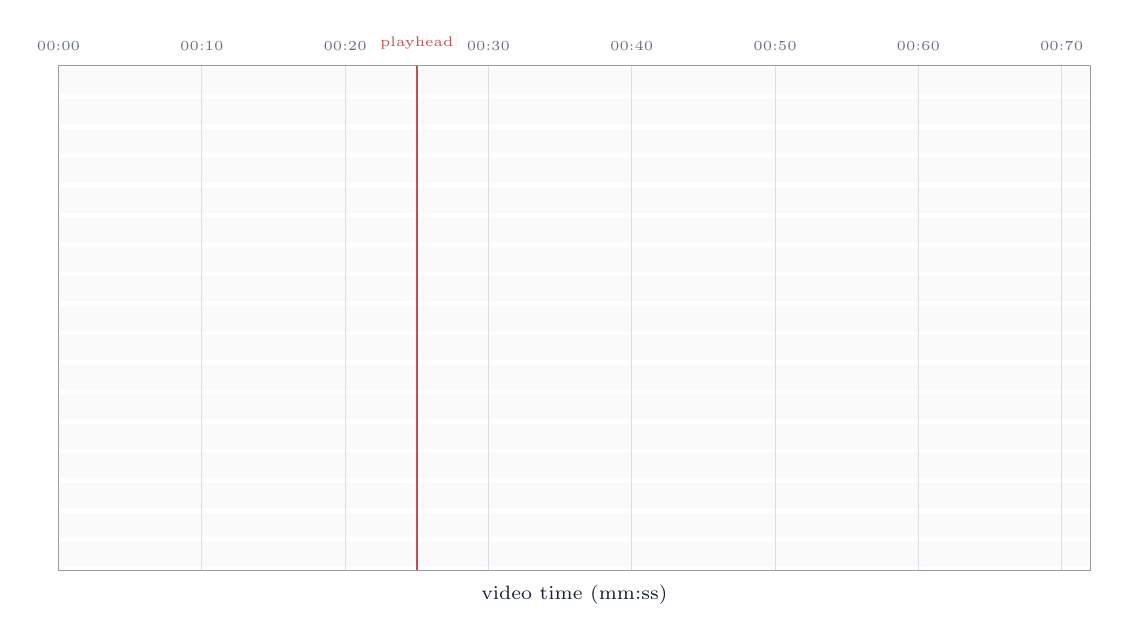
\begin{tikzpicture}[x=1.82mm,y=-3.75mm]
  % Row bands and time grid.
  \foreach \row in {0,...,16}{
    \fill[black!2] (0,\row-0.42) rectangle (72,\row+0.42);
  }
  \foreach \time in {0,10,...,70}{
    \draw[LLGrid,line width=0.35pt] (\time,-0.55) -- (\time,16.55);
    \node[font=\tiny,text=LLMuted,anchor=south] at (\time,-0.72)
      {\ifnum\time<10 00:0\time\else 00:\time\fi};
  }

  % Auto-generated transcription of the supplied visibility-timeline screenshot.
% Times are recovered from the displayed pixel positions and are illustrative.
\lltimelabel{0}{Paints and Lacquers}{LLPaints}
\llsegment{0}{16.33}{17.82}{LLPaints}
\llsegment{0}{20.14}{20.68}{LLPaints}
\llsegment{0}{26.87}{30.20}{LLPaints}
\llsegment{0}{33.06}{34.56}{LLPaints}
\llsegment{0}{39.80}{41.70}{LLPaints}
\llsegment{0}{68.98}{69.46}{LLPaints}
\llsegment{0}{70.41}{71.36}{LLPaints}
\lltimelabel{1}{MCP}{LLMcp}
\llsegment{1}{9.66}{10.14}{LLMcp}
\llsegment{1}{16.33}{17.28}{LLMcp}
\llsegment{1}{25.92}{27.82}{LLMcp}
\llsegment{1}{41.29}{42.18}{LLMcp}
\llsegment{1}{63.67}{64.22}{LLMcp}
\lltimelabel{2}{KLG}{LLKlg}
\llsegment{2}{16.39}{17.28}{LLKlg}
\llsegment{2}{19.66}{20.68}{LLKlg}
\llsegment{2}{26.87}{28.30}{LLKlg}
\llsegment{2}{29.73}{30.68}{LLKlg}
\llsegment{2}{34.01}{34.49}{LLKlg}
\llsegment{2}{41.22}{41.70}{LLKlg}
\llsegment{2}{70.41}{71.84}{LLKlg}
\lltimelabel{3}{Romantica}{LLRomantica}
\llsegment{3}{4.83}{6.80}{LLRomantica}
\llsegment{3}{7.76}{10.61}{LLRomantica}
\llsegment{3}{16.80}{18.30}{LLRomantica}
\llsegment{3}{21.63}{23.06}{LLRomantica}
\llsegment{3}{31.63}{32.18}{LLRomantica}
\llsegment{3}{45.51}{45.99}{LLRomantica}
\llsegment{3}{47.41}{47.96}{LLRomantica}
\llsegment{3}{65.17}{65.65}{LLRomantica}
\lltimelabel{4}{Bartercard}{LLBarter}
\llsegment{4}{16.39}{18.30}{LLBarter}
\llsegment{4}{28.78}{29.73}{LLBarter}
\llsegment{4}{32.59}{33.54}{LLBarter}
\llsegment{4}{39.80}{41.16}{LLBarter}
\llsegment{4}{43.61}{44.01}{LLBarter}
\llsegment{4}{45.51}{45.92}{LLBarter}
\llsegment{4}{47.41}{47.96}{LLBarter}
\llsegment{4}{70.41}{70.82}{LLBarter}
\lltimelabel{5}{Fairway}{LLFairway}
\llsegment{5}{16.33}{17.28}{LLFairway}
\llsegment{5}{32.59}{34.56}{LLFairway}
\llsegment{5}{35.99}{36.94}{LLFairway}
\llsegment{5}{39.32}{41.70}{LLFairway}
\lltimelabel{6}{Floor Tonic}{LLFloorTonic}
\llsegment{6}{4.83}{6.33}{LLFloorTonic}
\llsegment{6}{31.63}{32.18}{LLFloorTonic}
\lltimelabel{7}{ASC Group}{LLAsc}
\llsegment{7}{16.33}{17.28}{LLAsc}
\llsegment{7}{19.66}{20.20}{LLAsc}
\llsegment{7}{34.01}{34.56}{LLAsc}
\llsegment{7}{40.75}{42.18}{LLAsc}
\lltimelabel{8}{Ellgren}{LLEllgren}
\llsegment{8}{4.83}{8.23}{LLEllgren}
\llsegment{8}{16.80}{18.30}{LLEllgren}
\llsegment{8}{31.63}{32.18}{LLEllgren}
\lltimelabel{9}{ATM Hospitality}{LLAtm}
\llsegment{9}{16.80}{18.30}{LLAtm}
\llsegment{9}{28.78}{29.25}{LLAtm}
\llsegment{9}{33.06}{33.61}{LLAtm}
\llsegment{9}{39.80}{40.75}{LLAtm}
\llsegment{9}{45.51}{45.99}{LLAtm}
\llsegment{9}{47.41}{47.96}{LLAtm}
\lltimelabel{10}{Aon}{LLAon}
\llsegment{10}{4.83}{9.59}{LLAon}
\llsegment{10}{16.80}{17.21}{LLAon}
\llsegment{10}{19.66}{20.61}{LLAon}
\lltimelabel{11}{MNA Support}{LLMnaSupport}
\llsegment{11}{16.80}{17.21}{LLMnaSupport}
\llsegment{11}{31.63}{32.18}{LLMnaSupport}
\lltimelabel{12}{CCH}{LLCch}
\llsegment{12}{31.63}{32.59}{LLCch}
\llsegment{12}{47.41}{47.96}{LLCch}
\lltimelabel{13}{Chadlaw}{LLChadlaw}
\lltimelabel{14}{MNA Cladding}{LLMnaClad}
\llsegment{14}{9.66}{10.14}{LLMnaClad}
\llsegment{14}{16.80}{17.82}{LLMnaClad}
\lltimelabel{15}{EM Workwear}{LLEm}
\llsegment{15}{16.33}{18.30}{LLEm}
\llsegment{15}{20.14}{20.68}{LLEm}
\lltimelabel{16}{Top Notch}{LLTopNotch}


  % Interface playhead retained as an inspectability cue.
  \draw[LLRed,line width=0.8pt] (25,-0.58) -- (25,16.55);
  \node[font=\tiny,text=LLRed,anchor=south] at (25,-0.78) {playhead};

  \draw[LLNavy!45,line width=0.45pt] (0,-0.55) rectangle (72,16.55);
  \node[font=\scriptsize,text=LLNavy] at (36,17.35) {video time (mm:ss)};
\end{tikzpicture}
}
  \caption[Prototype brand-level visibility timeline]{Prototype brand-level
  visibility timeline. Each bar represents one displayed visibility segment;
  its position and extent are encoded directly as editable TikZ coordinates.}
  \label{fig:timeline-tikz}
\end{figure}

\end{document}
